%!TEX root = ../thesis.tex
%*******************************************************************************
%****************************** Third Chapter *********************************
%*******************************************************************************

\chapter{Modelling}\label{Modelling}

\ifpdf
    \graphicspath{{Chapter3/Figs/Raster/}{Chapter3/Figs/PDF/}{Chapter3/Figs/}}
\else
    \graphicspath{{Chapter3/Figs/Vector/}{Chapter3/Figs/}}
\fi


\section{Minimal Spanning Tree}\label{Minimal Spanning Tree}
The initial approach taken was to solve this problem as though it was a minimal spanning tree. This means having a series of building nodes on a standard $x,y$ graph and connecting all of them in such a way that means the shortest path is found between the nodes.

\subsection{Modelling Connections}\label{Modelling Connnections}
The first definition required is defining connections between nodes; this is done by using a boolean value. If a connection exists between two points $i$ and $j$, it is true, otherwise it is false.
\[
n_{ij} = \{0,1\}
\]
\subsection{Mathematical Maximum Number of Required Connections}\label{Mathematical Maximum Number of Required Connections}
When dealing with an optimiser, it is important to define exactly what is needed. In this case, the objective function\footnote{See Section \ref{Objective Function} for more information on the Objective Function} of the optimizer is to minimize the number of connections between nodes and the distance travelled by these connections however, we want the exact number of nodes required to connect all nodes in the graph. If this constraint is not implemented for this solution, the optimiser would simply draw no connections as that is the most effective solution.
In this case, the maths determining the exact number of connections required is quite simple.

\begin{figure}[H]
    \centering
    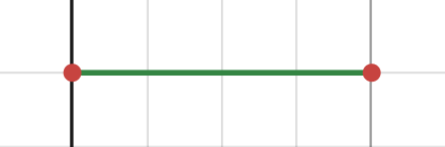
\includegraphics[width=0.35\linewidth]{twonodes.png}
    \caption{One connection between two nodes on a graph}
    \label{fig:Two Nodes}
\end{figure}

Looking at the above figure, it is easy to determine that a single connection is required to connect two nodes.

\begin{figure}[H]
    \centering
    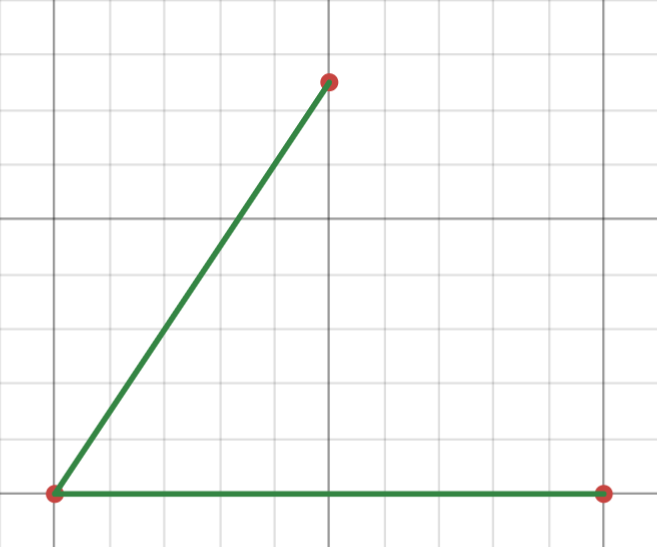
\includegraphics[width=0.30\linewidth]{threenodes.png}
    \caption{Two connections between three nodes on a graph}
    \label{fig:Three Nodes}
\end{figure}

Similarly, in the above figure, only two connections are required to connect three nodes.
\begin{figure}[H]
    \centering
    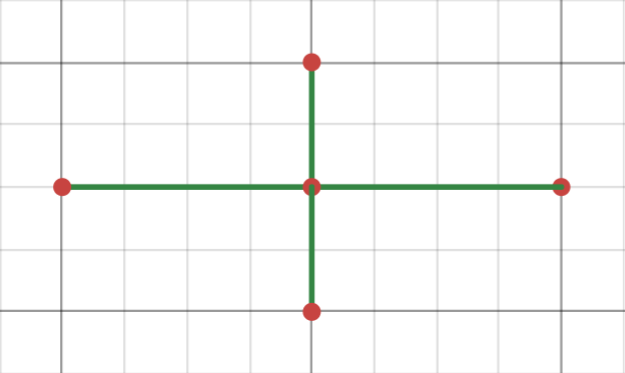
\includegraphics[width=0.35\linewidth]{fivenodes.png}
    \caption{Four connections between five nodes on a graph}
    \label{fig:Five Nodes}
\end{figure}


This paradigm scales indeterminately: where $N-1$ nodes are required to connect $N$ nodes.
\newline
This means modelling the exact number of connections required to connect all the nodes in the graph is simple: $N-1$ connections are required to connect $N$ nodes.
\[
\sum_{i,j \in B}n_{ij} =N -1
\]
\subsection{Breaking Symmetry}\label{Breaking Symmetry}
In order to ensure the mathematics of $N-1$ connections being required remains true, it is required to ensure duplicate paths can not exist. For example, if there is a connection between $i$ and $j$, a connection between $j$ and $i$ must not also exist as these would be different but symmetric according to the model. This is enforced by introducing another constraint upon the model.
\newline
\[
n_{ij} + n_{ji} \le 1 \quad\forall i,j\in B, i \neq j
\]
This constraint means that for a connection between $i$ and $j$, the symmetric connection cannot be made between $j$ and $i$.
\subsection{Distance Between Two Points}\label{Distance Between Two Points}
Calculating the distance between two points on the graph is the next mathematical constraint to be introduced into the model, as this is required in order to find the most efficient solution. This is relatively rudimentary mathematics and as such is simple to implement using the Pythagorean Theorem.
\[
d_{ij}=\sqrt{(x_i-x_j)^2 +(y_i-y_j)^2} \quad \forall i,j\in B, i\neq j
\]
\subsection{Ensuring At Least One Connection For Each Node}\label{Ensuring At Least One Connection For Each Node}
The final constraint to include before the objective function is that each node must have at least one connection to or from it: this ensures that every node is connected to the graph.

With the knowledge that the graph is undirected this is similar to the constraint introduced in \ref{Breaking Symmetry}.
\[
\sum_{i,j \in B} ( n_{ij} + n_{ji}) \geq 1, \quad i\neq j
\]

\subsection{Objective Function}\label{Objective Function}
Finally, the Objective Function is added to the optimiser. The objective function defines exactly what the optimiser is seeking to maximise or minimise. In this case, the optimiser's goal should be to minimise the distance travelled between the nodes - thus reducing the cost when they are all connected. The fact of connections existing between every node is already defined within the constraints and notation and so the objective function deals solely with minimising distance travelled between the nodes where each connection has an associated cost $d_{ij}$.\footnote{At this stage of the model, there exists an equivalency between distance and cost.}
\[
\min \sum_{i,j\in B}d_{ij}\cdot n_{ij}
\]
In the above function, if an edge $n_{ij}$ exists (is true), its distance is added to the total sum of distances and the optimisers goal is to minimise this total sum of distances travelled between the nodes.

\begin{figure}[H]
    \centering
    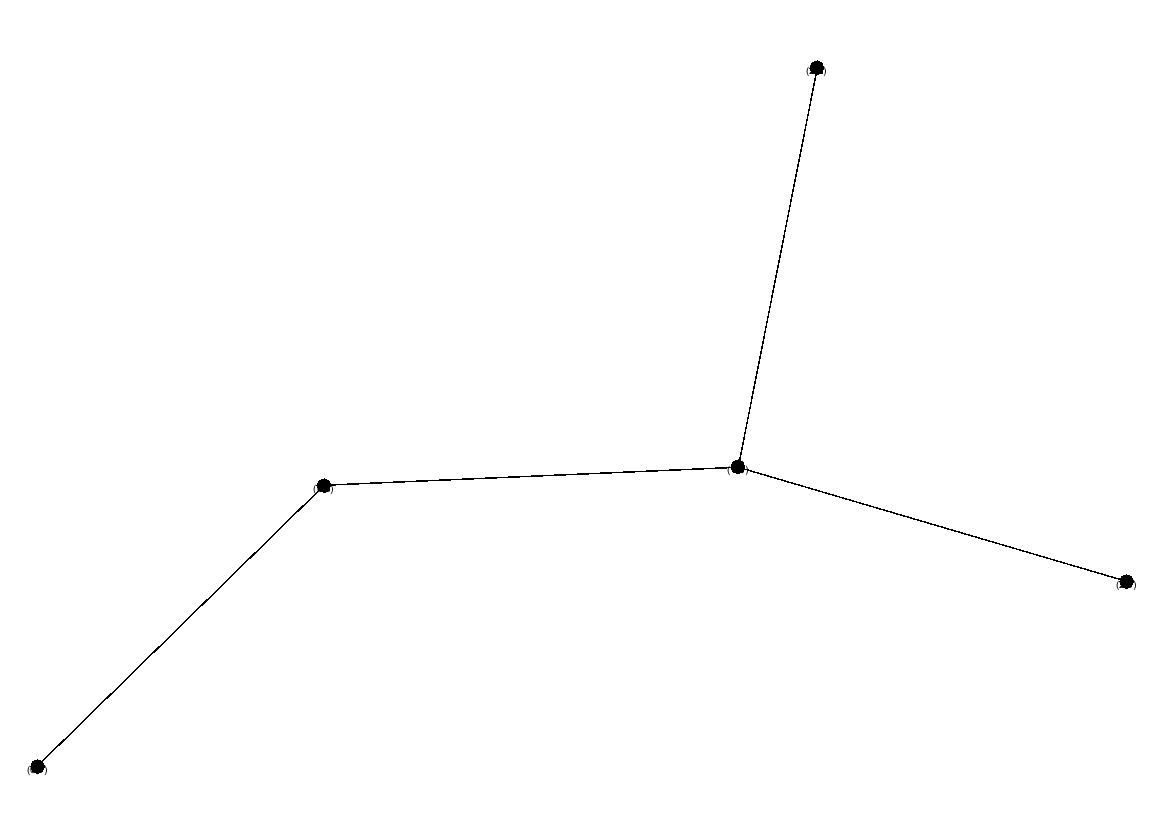
\includegraphics[width=0.35\linewidth]{protoAworking.png}
    \caption{A fully connected Minimal Spanning Tree}
    \label{fig:Fully connected Minimal Spanning Tree}
\end{figure}

The complete solution outlined functions perfectly for smaller, more dense graphs, however as the optimiser deals with more nodes across a larger graph the optimiser begins to form subtours.

\begin{figure}[H]
    \centering
    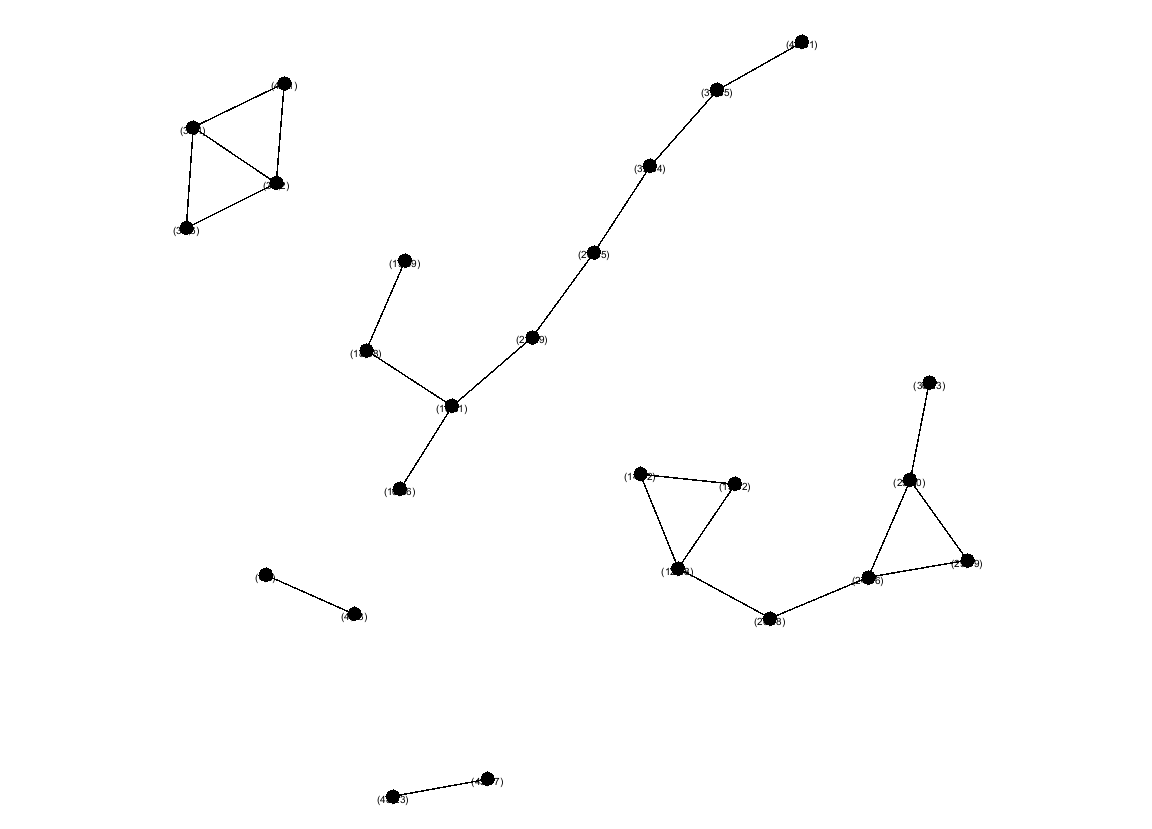
\includegraphics[width=0.35\linewidth]{subtours.png}
    \caption{A graph containing subtours}
    \label{fig:subtours}
\end{figure}

This is due to it being more cost-efficient for smaller cycles to be constructed by the optimiser while abiding by the constraints defined as opposed to connecting distant nodes to the greater graph.

\section{Reducing Subtours}
There are a number of ways designed to reduce subtours in a tree like this. The primary solutions that exist in the existing literature are designed to aid in solving the Travelling Salesman Problem \citep{Hoffman2013}. While the TSP seeks to form a Hamiltonian Cycle as opposed to a tree, it could be possible to use similar mathematics as a solution to the proposed problem.

\subsection{Subtour Elimination Constraints (SECs)}
Subtour Elimination Constraints are the standard method for reducing subtours in Mixed Integer Programming formulations. \citep{Clautiaux2025}
\subsubsection{Exponential SECs}\label{ExpSEC}
Exponential SECs are the classical form for solving such a problem \citep{tsp_2007}. The goal is to find a minimum-cost tour that visits every city exactly once, forming a Hamiltonian Cycle. Even simply forcing every node in the array to have just two edges can return disconnected subtours.
\[
\sum_{j\in B}n_{ij} = 2
\]
For example, given three nodes A, B, and C: it would be valid to return $A\rightarrow B \rightarrow C$ as a valid solution even if there were other nodes in the system as each node conforms to a degree of two.
\newline
As such, constraints can be added to forbid any cycle that visits only a strict subset of cities.
\[\text{Let }S\subset B \text{, where }2\leq |S|<|B|\]
\[\text{Let }E(S) = {(i,j)\in B:i,j\in S}\text{: all edges fully hosted inside the subset $S$.}\]
A cycle over $|S|$ nodes contains exactly $|S|$ edges. So if the sum of $n_{ij}$ over edges in $E(S)$ is $|S|$, a subtour is implied - a full cycle on $|S|$. This constraint says that $|S|$ edges cannot be used entirely with a set of size |$S$|, at most only $|S|-1$ \citep{Petrica_2007}. Therefore, the cycle is broken and the subtour is forced to extend outside $S$.
However, there are $2^n-2n+1$ such subsets that exist in a set of size $n$ that is exponential in $n$ and as such it is infeasible to add these upfront. \citep{Pferschy_2016}

\subsubsection{Miller-Tucker-Zemlin (MTZ) Constraints}\label{MTZ}
The purpose of MTZ constraints is to eliminate subtours without listing all possible subsets. MTZ achieves this by introducing an ordering system over the cities, making subtours logically impossible. \citep{MTZ_Constraints}\newline
Firstly, degree constraints are introduced. Exactly one departure and one arrival per city:
\[
\sum n_{ij} = 1 \quad\forall i,j\in E
\]
\[
\sum n_{ji} = 1 \quad\forall i,j\in E
\]
However this still allows subtours.\newline
MTZ then introduces the continuous variables $u_i \in [1, |B| - 1]$ for $i \in \{2,...,|B|\}$. $u_i$ encodes the order in which city $i$ is visited. City 1 is considered the starting city so $u_1=0$ is fixed. These variables are used to enforce a consistent visit order as a requirement which cannot be met if a subtour exists. The final MTZ constraint is then introduced:
\[
u_i-u_j+(|B|-1)n_{ij}\leq |B|-2 \quad\forall i,j\in \{2,...,|B|\}, i\neq j
\]
Subtours cannot exist in an ordered system like this and so this blocks them implicitly.\newline
While this system disallows subtours/cycles and does not have as high of a time and memory complexity as Exponential SECs, it can still be memory-heavy for a large B. Similarly, it exists in polynomial time which is still not ideal. The final factor which disallows this system completely is that it only allows one departure per node which is not always the optimal solution when constructing a tree as opposed to a Hamiltonian Cycle where it is always optimal.

\subsubsection{Lazy Constraints (Dynamic SECs)}\label{Lazy Constraints}
In the classical SEC formulation mentioned in Section \ref{ExpSEC}:
\[
\sum_{i,j\in B}n_{ij}\leq |S| - 1\quad\forall S\in V, 2\leq|S|<|B|
\]
This set of constraints is exponential which makes adding all of them impractical. Lazy constraints aim to fix this by adding only the violated subtour constraints dynamically when testing if a solution is valid. When the solver finds a feasible integer solution, a subtour detection algorithm is run. If a subtour is found, the subtour is identified and the following constraint is added:
\[
\sum_{i,j\in B}n_{ij}\le |S|
\]
This cuts off the invalid solution. This is repeated until an optimal subtour-free solution is found. This functions better than an MTZ as it starts small however is harder to implement as a callback is required in code. \citep{Pferschy_2016}


\subsection{Implementing Flow}\label{Implementing Flow}
The final potential solution to review is the implementation of a water-flow based system to remove subtours. This is similar to the MTZ approach to removing subtours however instead of order being counted, the flow of $n-1$ units of a single commodity/variable passed through each node is modelled. The objective function would be the same as mentioned in Section \ref{Objective Function}.\newline
In the context of the TSP, the first constraint would be that each node has one incoming and one outgoing edge.
\[
\text{For all nodes $i$:}
\]
\[
\sum_{j\neq i}n_{ij} = 1 \quad \forall j\in B
\]
\[
\sum_{j\neq i}n_{ji} = 1 \quad \forall j\in B
\]
This would ensure the commodity flows correctly around the circuit. The next constraint to declare is a flow conservation constraint, similar to Kerchoff's Voltage Laws in circuits which state "in any closed loop network being driven by a voltage source, the total voltage around the loop is equal to the sum of all the voltage drops within the same loop" which is equal to zero. \citep{alexander_2012_fundamentals}

\begin{itemize}
    \item At node 1: Send out $n-1$ units of the commodity variable
    \[
    \sum_{j \ne 1} f_{1j} = n - 1
    \]

    \item At each node $i \in B$, except node 1, the output must be exactly the input $- 1$
    \[
    \sum_{j \ne i} f_{ji} - \sum_{j \ne i} f_{ij} = 1
    \]
\end{itemize}
This means node $i$ receives on unit, and passes on the rest.
Finally, we enforce that flow only travels along edges that exist.
\[
f_{ij}\leq (|B|-1)n_{ij} \quad\forall i\neq j
\]
This enforces that flow can only go edges that exist, if $n_{ij} = 0$, then $f_{ij}=0$. If $n_{ij}=1$, max flow on it is $|B|-1$.
\newline\newline
This implementation would work perfectly for the proposed system: not just due to it's removal of subtours however also due it's inclusion of the commodity that is carried between nodes. This "flow" commodity can be perfectly modelled to match the water pressure water requirements.

\subsubsection{Adaptation For Use Within The Model}
Adapting this model to fit the solution is relatively straight-forward as a result of it's logical fit with the exception of the degree constraints. Currently, in order to remove subtours from the TSP, each node is limited to a degree constraint of two - one edge in and one edge out - however this is not suitable when trying to model a tree as it can be more efficient to have one node connecting to multiple nearby nodes.\newline\newline
Contrarily, the commodity variable used to remove subtours can be perfectly modelled to match water pressure. This means that ensuring each node receives it's required pressure will successfully remove all subtours. This also means each node can consume recieve and consume more than a single unit of the commodity variable. In order to mathematically model connections between nodes as pipes, I must place the nodes on a grid so that pipes can be routed in the most efficient way possible.


The function $f_{ij}$ stores the water pressure between two given nodes $i$ and $j$ as opposed to the commodity variable referenced in \ref{Implementing Flow}.

\section{A Flow-Based System}\label{A Flow-Based System}
\subsection{Establishing a Grid and Source Nodes}
A flow-based system can be implemented using the information gained from the research in Section \ref{Implementing Flow}. Firstly, the nodes are defined on a grid with a series of intermediate/junction nodes as opposed to just the building nodes. For example, given a $5x5$ graph with building nodes at $(3,4)$ and $(2,1)$, all the remaining nodes in the graph must be populated with blank junction nodes. These will facilitate the flow of water through these points towards the building nodes.\newline
It is then required to introduce a source node that will pump water throughout the system. For the purposes of modelling a system, at this stage, the maximum pressure flow of the singular source pump will be set to the total pressure required throughout the system. At a later point in the development process this will be changed to match real-life pressure numbers.
\[
P_{total}= \sum_{i\in B}D_i \quad\text{where $D_i$ represents the pressure demand at building $i$}
\]
\subsection{Node Links and Flow Links}\label{nodeandflowlinks}
Similar to the system in Section \ref{Minimal Spanning Tree}, the existence of a pipe between two nodes will be measured by $n_{ij}$ however, in this instance, the nodes referenced can be junctions, sources and building nodes. Furthermore, similar to the system researched and defined in Section \ref{Implementing Flow}, flow between any two nodes will be measured and stored in $f_{ij}$.
\subsection{Transfer of Flow}\label{flowonexistingedge}
Mathematically and logically, flow should only be allowed to travel through pipes, i.e. where edges exist in the graph. It is required to set an upper bound constraint on this flow: the maximum flow that can travel through pipes.
\[
f_{ij}\leq P_{total}\cdot n_{ij}, \quad\forall i,j \in B \text{ where $n_{ij}$ exists}
\]
This only allows flow to exist above zero when $n_{ij}$ is true, i.e. a pipe exists at that point, and limits flow to the maximum possible flow throughout the system.
\subsubsection{Adjacency}
It is important at this stage to consider where a connection $n_{ij}$ should be able exist. Logically, connections should only be able to be made between adjacent nodes. This will allow a logical flow to exist from a source node, through intermediate/junction nodes, and end at a building node. If this is not implemented at this stage, flow can just start at a source node and end at a building node with little consideration for the distance travelled.

\subsection{Flow Conservation}\label{flowconservation}
The final constraints to be added to this model before the objective function are the constraints which will enforce Flow Conservation i.e. the physics regarding how water will flow between nodes in this model. Sources are defined as a start point for water flow travelling through pipes between intermediate nodes until reaching their end-point at the building nodes.
\subsubsection{Source Nodes}
First is source nodes, these should have no inflow and should have an outflow equal to the source's capacity.\newline
Defining $x$ as the source node:
\[
\text{Inflow: }\sum_{i\neq x}f_{ix} = 0 \quad \forall i\in B
\]
\[
\text{Outflow: }\sum_{i\neq x}f_{xi}\leq P_x \quad \forall i\in B
\]
\subsubsection{Building Nodes}
For building nodes, there should be no outflow and they must receive at minimum their required flow - this could be minimised to be the exact required amount however at this stage receiving at least their required flow is appropriate for the model.\newline
Defining $x$ as the building node:
\[
\text{Inflow: }\sum_{i\neq x}f_{ix} \geq D_x \quad\forall i \in B
\]
\[
\text{Outflow: }\sum_{i\neq x}f_{xi} = 0 \quad\forall i \in B
\]

\subsubsection{Junction Nodes}
For junction nodes, the inflow must be equal to the outflow as they are simply connection points for pipes to travel through.
Defining $x$ as the junction node:
\[
\sum_{i\neq x} f_{ix}= \sum_{i\neq x}f_{xi} \quad\forall i \in B
\]

\subsection{Objective Function}
Finally, we define our objective function. Once again we are looking to minimise the distance travelled to reach every node and so this is defined the same as for solving the Minimal Spanning Tree in Section \ref{Objective Function}.
\[
\min\sum_{i,j\in B}d_{ij}\cdot n_{ij}
\]
\subsection{Removal of the Enforced Mathematical Maximal Number of Connections}
The final note to make on this implementation is the removal of the constraint $\sum_{i,j \in B}n_{ij} =N -1$, defined in Section \ref{Mathematical Maximum Number of Required Connections}, used to define the number of connections in order to ensure every building node was connecting to the graph. This must now be removed due to the inclusion of junctions as each pipe to an intermediate node would also count as a connection under the given constraint. Instead, it can now be assumed every building node is connected as a result of the flow-based system. The model is now constrained to ensure every node receives it's required water pressure. When this constraint is met, it is implied that every building node is connected to the wider graph.

\section{Optimising A Flow-Based System}
\subsection{Replacing the Distance Metric}\label{definingdistance}
At this stage, the optimisation algorithm tends towards many bends as opposed to straight lines when trying to reach a point.

% Side by side subfigures 
\begin{figure}[H]
    \begin{subfigure}{0.4\linewidth}\label{fig:Sinuous Line}
        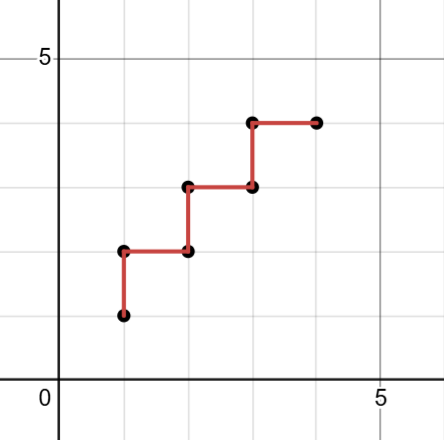
\includegraphics[width=\linewidth]{zig-zag.png}
        \caption{A sinuous line heading towards a point}
    \end{subfigure}
    \hfill
    \begin{subfigure}{0.4\linewidth}
        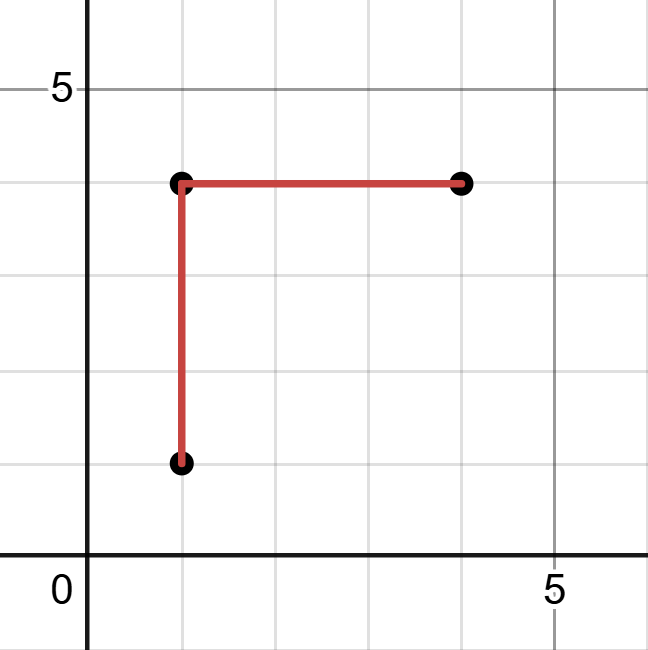
\includegraphics[width=\linewidth]{straightlinetoapoint.png}
        \caption{Straight lines heading towards a point}
    \end{subfigure}
        \caption{A comparison between two methods for connecting two points}
        \label{sinuousvszigzag}
\end{figure}

These two scenarios have the exact same cost value in the current implementation of the optimiser. However, when considering real-life factors, the approach taken in Figure 2.6.a is more expensive due to installing six pipes as opposed to just two pipes. This means that a method of allowing longer pipes and a method of incorporating pipe installation costs to the overall price calculation is required.

\subsubsection{$C_{ij}$ Formulation}\label{definingcost}
First is to define the new cost metric. The new metric is required to account for the base installation cost of a pipe whilst still scaling with distance.
\[
c_{ij} = (d_{ij} \cdot \alpha) + \beta
\]
\[
\text{where $\alpha$ represents the cost per unit of piping}
\]
\[
\text{and $\beta$ represents the base installation cost of a pipe.}
\]
Adding a higher base installation cost can further encourage less pipes to be used overall by making it cheaper to run a single pipe than many pipes.

\subsubsection{Restructuring the Objective Function}\label{finalobjfunc}
Next is to reformulate the Objective Function. The objective function is still to minimise the cost spent on piping however is required to account for the new cost metric. This means that the $d_{ij}$ metric in the objective function is replaced with the new cost metric and the function is reformulated to the following:
\[
\min\sum_{i,j\in B}c_{ij}\cdot n_{ij}
\]
This minimises the cost of each pipe as opposed to the distance spanned however, when considering the definition of $c_{ij}$, the cost still scales with distance.

\subsubsection{Pipes Along An Axis}
Currently, mathematically, the same amount of pipes would still be used in Figure \ref{sinuousvszigzag}(a) vs Figure \ref{sinuousvszigzag}(b) as pipes can only connect to adjacent nodes, i.e. be a single unit in length. To fix this, connections need to be allowed between parallel nodes not exclusively between adjacent nodes.

\begin{figure}[H]
    \begin{subfigure}{0.4\linewidth}
        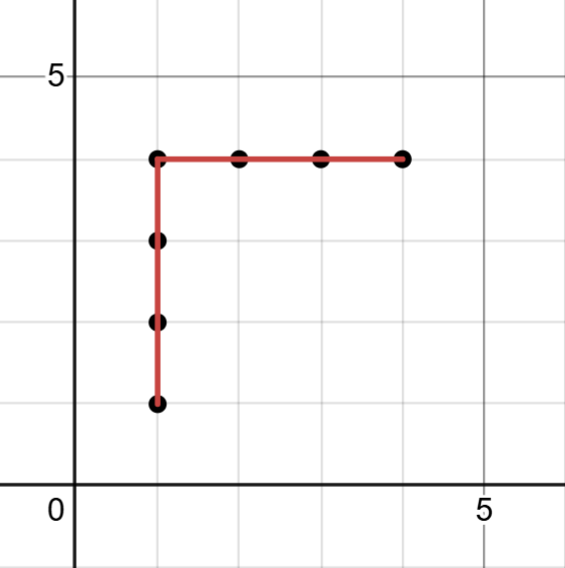
\includegraphics[width=\linewidth]{sixpoints.png}
        \caption{Six pipes across two axis}
    \end{subfigure}
    \hfill
    \begin{subfigure}{0.4\linewidth}
        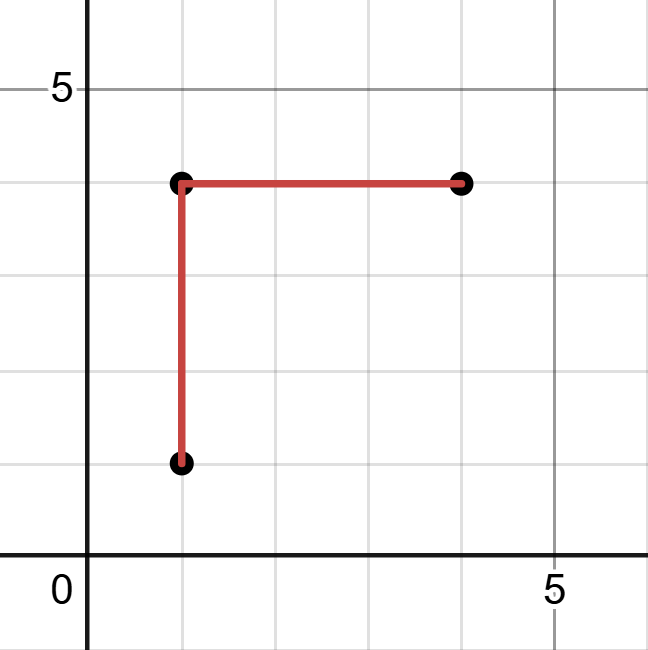
\includegraphics[width=\linewidth]{straightlinetoapoint.png}
        \caption{Two pipes across two axis}
    \end{subfigure}
        \caption{A comparison between the adjacent vs parallel connections when creating piping connections}
        \label{fig:6v2pipes}
\end{figure}
As clearly displayed in Figure \ref{fig:6v2pipes}, there is a significant difference when connections are allowed between parallel nodes as opposed to solely adjacent nodes as the pipe count goes from six pipes to two pipes.\newline\newline
This complete system now allows for Figure \ref{sinuousvszigzag}(b) to be cheaper than Figure \ref{sinuousvszigzag}(a) as it only uses two pipes as opposed to six. Furthermore, the inclusion of a base installation cost encourages the use of longer, straight runs of piping as opposed to a series of shorter pipes as would be preferred in the real-world.

\subsection{Altering Flow Conservation Laws}\label{alteringflowconservation}
Another decision made at this point is to allow the commodity flow variable to pass through buildings onto other nodes as opposed to forcibly end at buildings. This will be utilised when implementing into a wider system. To implement this the flow conversion laws are altered to allow outflow from buildings. It is important to note, buildings should still consume their required pressure.
\[
\text{Inflow: }\sum_{i\neq x}f_{ix} \geq D_x,\quad\forall i\in B,\quad\text{The inflow constraint remains unchanged.}
\]
The outflow flow constraint changes from the following where outflow is always zero.
\[
\text{Outflow: }\sum_{i\neq x}f_{xi} = 0,\quad \forall i \in B 
\]
The outflow constraint changes to the following, where the building consumes it's required flow and passes the remainder along the network.
\[
\text{Outflow: }\sum_{i\neq x}f_{xi} = \sum_{i\neq x}f_{ix} - D_x
\]
\[
\text{Simplified Outflow: }\sum_{i\neq x}f_{xi} = \text{Inflow} - D_x
\]

\section{Generating a Cartesian Grid}\label{Cartesian Grid}
When dealing with real-world elements, there is never a guarantee that the buildings will be arranged in such a way that they are exactly one unit apart. The distances between buildings can vary by the tiniest of fractions. As such, it is required to be able to generate a grid for any given layout of buildings. By solving this, it means that the grid size also does not have to be pre-determined and can be generated at the point the optimiser is required to run.\newline
The most efficient method to achieve this is through a mathematical construct known as a Cartesian Set. In Set Theory, the Cartesian Product of two sets, $A$ and $B$, is a new set formed by taking all possible ordered pairs where the first element of each pair is from set $A$ and the second element is from set $B$.\newline
This approach can be used here to generate every required node to connect a series of points. Suppose there are two sets:
\[
\text{Buildings = }\{(1,3), (2,4), (3,2)\} \text{ and Source = {(3,5)}}
\]
Building a Cartesian set for all these points would be the $x$ for every node against the $y$ of every node.

\[
\left\{
\begin{array}{c}
1 \\
2 \\
3 \\
\end{array}
\right\} \times
\left\{
\begin{array}{c}
3 \\
4 \\
2 \\
5
\end{array}
\right\} = \{(1,3), (1,4), (1,2), (1,5), (2,3), (2,4),(2,2), (2,5), (3,3),(3,4),(3,2),(3,5)\}
\]

Plotting these points on a graph would appear like so:
\begin{figure}[H]
    \centering
    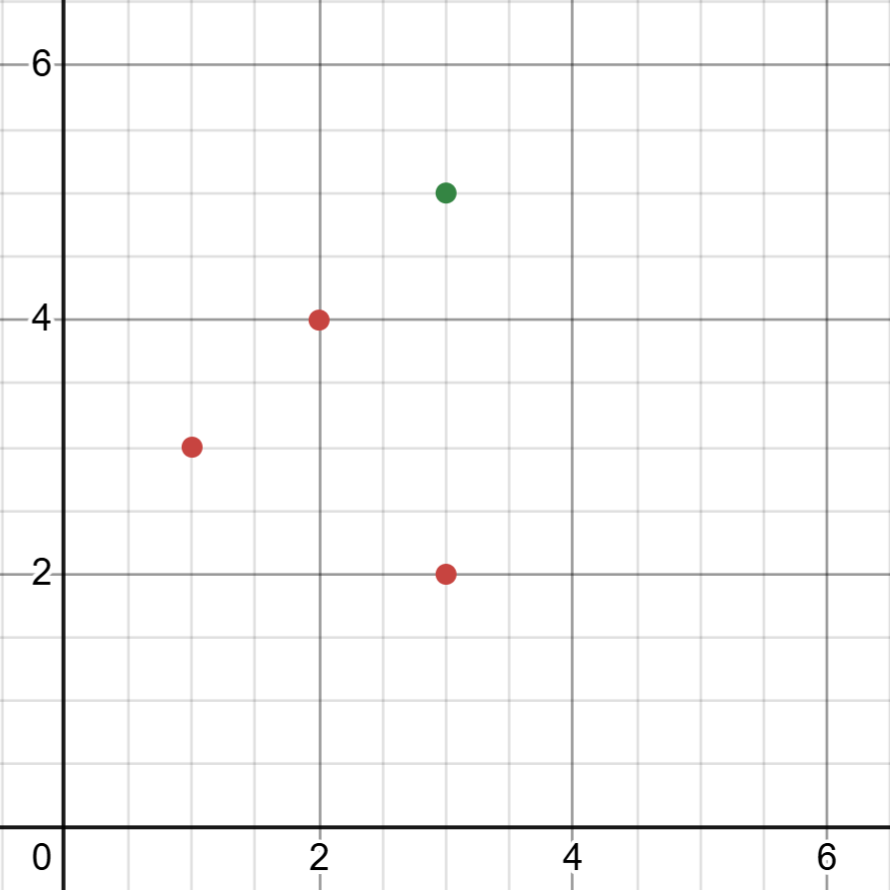
\includegraphics[width=0.4\linewidth]{cartesianpointsonagraph.png}
    \caption{A series of points on a graph}
    \label{fig:cartesianpointsonagraph}
\end{figure}
By taking the $x$ and $y$ of every node and building a Cartesian set it would look this, where every point of intersection is a coordinate in the Cartesian set for the model.
\begin{figure}[H]
    \centering
    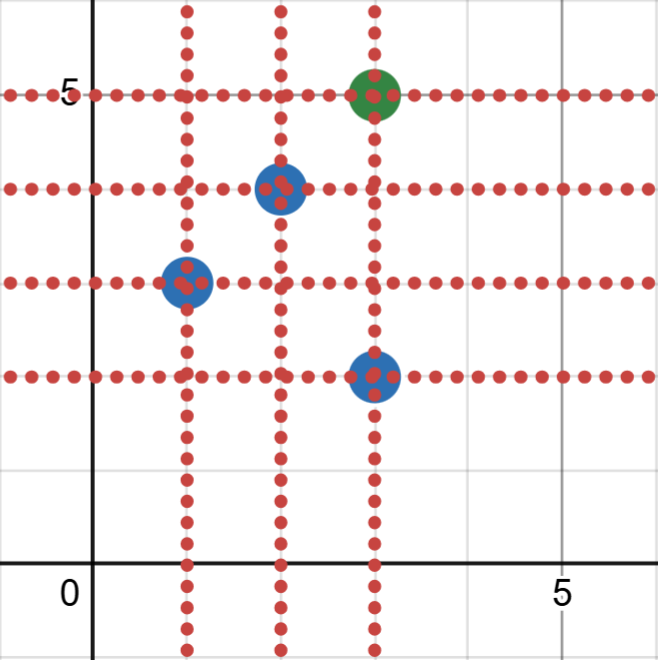
\includegraphics[width=0.4\linewidth]{cartesiansetonagraph.png}
    \caption{A Cartesian set represented on a graph}
    \label{fig:cartesiansetonagraph}
\end{figure}
Every point of intersection on Figure \ref{fig:cartesiansetonagraph} represents the whole Cartesian set. By plotting these, it is possible to build a set of intermediate nodes for any set of points, regardless of grid size or spacing between nodes.

\section{Multi-Source Flow}
A key point to highlight at this stage is that the modelled solver functions seamlessly for systems containing one or more source nodes. This functionality is possible due to the implementation of the commodity flow variable, which tracks and manges the flow of resources throughout the network. Unlike traditional single-source flow models, which often rely on a fixed origin point, the commodity flow formulation allows the solver to accommodate multiple input nodes, each which can contribute distinct quantities of flow into the system.\newline

This functionality is crucial as it ensures flexibility and scalability and is especially crucial in real-world applications, where resources may be injected from geographically distributed sources. For example, multiple pumping stations in a water supply system.\newline

The solver's ability to model multi-source systems accurately enhances its flexibility and improves its scalability. As the network grows in size and complexity, the solver retains its robustness, enabling it to adapt to varying topologies and supply scenarios without requiring fundamental changes to the model.

\begin{figure}
    \centering
    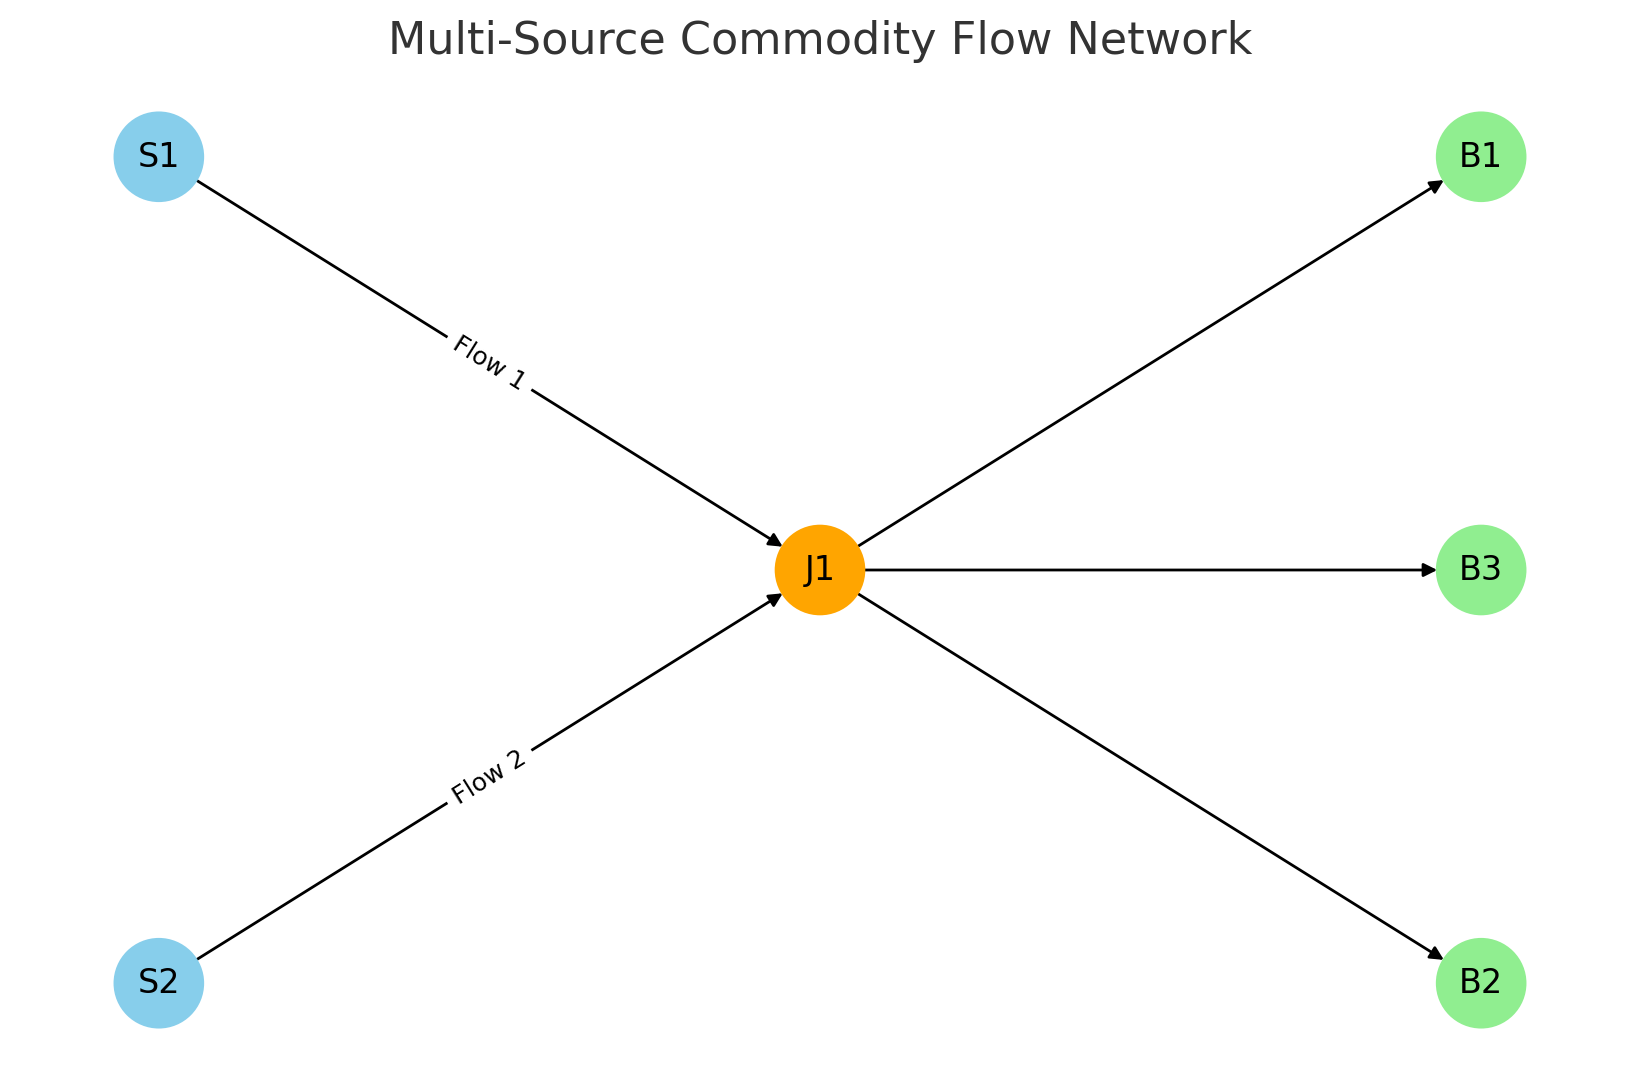
\includegraphics[width=0.5\linewidth]{multisource.png}
    \caption{A multi-source model showing the usage of multiple source nodes}
    \label{fig:multisource}
\end{figure}

